\documentclass[twoside]{book}

% Packages required by doxygen
\usepackage{fixltx2e}
\usepackage{calc}
\usepackage{doxygen}
\usepackage{graphicx}
\usepackage[utf8]{inputenc}
\usepackage{makeidx}
\usepackage{multicol}
\usepackage{multirow}
\PassOptionsToPackage{warn}{textcomp}
\usepackage{textcomp}
\usepackage[nointegrals]{wasysym}
\usepackage[table]{xcolor}

% Font selection
\usepackage[T1]{fontenc}
\usepackage{mathptmx}
\usepackage[scaled=.90]{helvet}
\usepackage{courier}
\usepackage{amssymb}
\usepackage{sectsty}
\renewcommand{\familydefault}{\sfdefault}
\allsectionsfont{%
  \fontseries{bc}\selectfont%
  \color{darkgray}%
}
\renewcommand{\DoxyLabelFont}{%
  \fontseries{bc}\selectfont%
  \color{darkgray}%
}
\newcommand{\+}{\discretionary{\mbox{\scriptsize$\hookleftarrow$}}{}{}}

% Page & text layout
\usepackage{geometry}
\geometry{%
  a4paper,%
  top=2.5cm,%
  bottom=2.5cm,%
  left=2.5cm,%
  right=2.5cm%
}
\tolerance=750
\hfuzz=15pt
\hbadness=750
\setlength{\emergencystretch}{15pt}
\setlength{\parindent}{0cm}
\setlength{\parskip}{0.2cm}
\makeatletter
\renewcommand{\paragraph}{%
  \@startsection{paragraph}{4}{0ex}{-1.0ex}{1.0ex}{%
    \normalfont\normalsize\bfseries\SS@parafont%
  }%
}
\renewcommand{\subparagraph}{%
  \@startsection{subparagraph}{5}{0ex}{-1.0ex}{1.0ex}{%
    \normalfont\normalsize\bfseries\SS@subparafont%
  }%
}
\makeatother

% Headers & footers
\usepackage{fancyhdr}
\pagestyle{fancyplain}
\fancyhead[LE]{\fancyplain{}{\bfseries\thepage}}
\fancyhead[CE]{\fancyplain{}{}}
\fancyhead[RE]{\fancyplain{}{\bfseries\leftmark}}
\fancyhead[LO]{\fancyplain{}{\bfseries\rightmark}}
\fancyhead[CO]{\fancyplain{}{}}
\fancyhead[RO]{\fancyplain{}{\bfseries\thepage}}
\fancyfoot[LE]{\fancyplain{}{}}
\fancyfoot[CE]{\fancyplain{}{}}
\fancyfoot[RE]{\fancyplain{}{\bfseries\scriptsize Generated on Thu Oct 12 2017 11\+:42\+:57 for My Project by Doxygen }}
\fancyfoot[LO]{\fancyplain{}{\bfseries\scriptsize Generated on Thu Oct 12 2017 11\+:42\+:57 for My Project by Doxygen }}
\fancyfoot[CO]{\fancyplain{}{}}
\fancyfoot[RO]{\fancyplain{}{}}
\renewcommand{\footrulewidth}{0.4pt}
\renewcommand{\chaptermark}[1]{%
  \markboth{#1}{}%
}
\renewcommand{\sectionmark}[1]{%
  \markright{\thesection\ #1}%
}

% Indices & bibliography
\usepackage{natbib}
\usepackage[titles]{tocloft}
\setcounter{tocdepth}{3}
\setcounter{secnumdepth}{5}
\makeindex

% Hyperlinks (required, but should be loaded last)
\usepackage{ifpdf}
\ifpdf
  \usepackage[pdftex,pagebackref=true]{hyperref}
\else
  \usepackage[ps2pdf,pagebackref=true]{hyperref}
\fi
\hypersetup{%
  colorlinks=true,%
  linkcolor=blue,%
  citecolor=blue,%
  unicode%
}

% Custom commands
\newcommand{\clearemptydoublepage}{%
  \newpage{\pagestyle{empty}\cleardoublepage}%
}


%===== C O N T E N T S =====

\begin{document}

% Titlepage & ToC
\hypersetup{pageanchor=false,
             bookmarks=true,
             bookmarksnumbered=true,
             pdfencoding=unicode
            }
\pagenumbering{roman}
\begin{titlepage}
\vspace*{7cm}
\begin{center}%
{\Large My Project \\[1ex]\large 0.\+1 }\\
\vspace*{1cm}
{\large Generated by Doxygen 1.8.8}\\
\vspace*{0.5cm}
{\small Thu Oct 12 2017 11:42:57}\\
\end{center}
\end{titlepage}
\clearemptydoublepage
\tableofcontents
\clearemptydoublepage
\pagenumbering{arabic}
\hypersetup{pageanchor=true}

%--- Begin generated contents ---
\chapter{Class Index}
\section{Class List}
Here are the classes, structs, unions and interfaces with brief descriptions\+:\begin{DoxyCompactList}
\item\contentsline{section}{\hyperlink{class_application}{Application} \\*Ensemble des éléments et action du menu principal }{\pageref{class_application}}{}
\item\contentsline{section}{\hyperlink{class_etudiant}{Etudiant} \\*Permet d'interagir avec les élèves, avoir leurs noms etc.. }{\pageref{class_etudiant}}{}
\item\contentsline{section}{\hyperlink{class_evaluation}{Evaluation} \\*Permet de créer et d'interagir avec des évaluations }{\pageref{class_evaluation}}{}
\item\contentsline{section}{\hyperlink{class_matiere}{Matiere} \\*Permet de créer et d'interagir avec les matières }{\pageref{class_matiere}}{}
\item\contentsline{section}{\hyperlink{class_note}{Note} \\*Permet de créer des notes en les lien avec les étudiants }{\pageref{class_note}}{}
\item\contentsline{section}{\hyperlink{class_section}{Section} \\*Permet le liens avec \hyperlink{class_section}{Section} pour en utiliser des éléments }{\pageref{class_section}}{}
\end{DoxyCompactList}

\chapter{File Index}
\section{File List}
Here is a list of all files with brief descriptions\+:\begin{DoxyCompactList}
\item\contentsline{section}{\hyperlink{application_8h}{application.\+h} }{\pageref{application_8h}}{}
\item\contentsline{section}{\hyperlink{bulletin_8h}{bulletin.\+h} }{\pageref{bulletin_8h}}{}
\item\contentsline{section}{\hyperlink{etudiant_8h}{etudiant.\+h} }{\pageref{etudiant_8h}}{}
\item\contentsline{section}{\hyperlink{evaluation_8h}{evaluation.\+h} }{\pageref{evaluation_8h}}{}
\item\contentsline{section}{\hyperlink{matiere_8h}{matiere.\+h} }{\pageref{matiere_8h}}{}
\item\contentsline{section}{\hyperlink{note_8h}{note.\+h} }{\pageref{note_8h}}{}
\item\contentsline{section}{\hyperlink{section_8h}{section.\+h} }{\pageref{section_8h}}{}
\end{DoxyCompactList}

\chapter{Class Documentation}
\hypertarget{class_application}{\section{Application Class Reference}
\label{class_application}\index{Application@{Application}}
}


ensemble des éléments et action du menu principal  




{\ttfamily \#include $<$application.\+h$>$}

\subsection*{Public Member Functions}
\begin{DoxyCompactItemize}
\item 
vector$<$ \hyperlink{class_matiere}{Matiere} $>$ $\ast$ \hyperlink{class_application_adf59d6a0ecdc83288605c6a1a952bdd0}{get\+Vect\+Matiere\+App} ()
\item 
\hyperlink{class_application_afa8cc05ce6b6092be5ecdfdae44e05f8}{Application} ()
\item 
void \hyperlink{class_application_a68965449404743bf1add056784d6cf81}{run} ()
\end{DoxyCompactItemize}
\subsection*{Private Member Functions}
\begin{DoxyCompactItemize}
\item 
void \hyperlink{class_application_aef7daa6aaa1eefe73663d70bf3b86d4c}{afficher\+Menu} ()
\item 
char \hyperlink{class_application_af37c055a9dde1f5006413ab7f8ddc2ce}{saisie\+Controle\+Du\+Choix\+Utilisateur} ()
\item 
void \hyperlink{class_application_acb082ff0c42e6d4a906c589a31c22fc3}{realisation\+Action\+Correspondante\+Au\+Choix} (char le\+Choix)
\item 
void \hyperlink{class_application_a63ca3c3beb6f3a62739d0a2005546758}{afficher\+Sections} ()
\item 
void \hyperlink{class_application_a9f05868c8936a996e1b4e7a04b3e4c9d}{creer\+Section} ()
\item 
void \hyperlink{class_application_a3cfad12ed5d0c2b6a1468aeec5e26c2b}{gerer\+Section} ()
\item 
void \hyperlink{class_application_a9cae102801b3c14a5a0e85123829ef25}{afficher\+Matieres} ()
\item 
void \hyperlink{class_application_a9d2b9b0edc784f4388b51cbc84c4de8c}{creer\+Matiere} ()
\end{DoxyCompactItemize}
\subsection*{Private Attributes}
\begin{DoxyCompactItemize}
\item 
vector$<$ \hyperlink{class_section}{Section} $>$ \hyperlink{class_application_a689a25902c2e34e61bdd122d4c92d941}{vect\+Section}
\item 
vector$<$ \hyperlink{class_matiere}{Matiere} $>$ \hyperlink{class_application_ac5a9a7ed9aab9411814d9cd53af9175d}{vect\+Matiere}
\end{DoxyCompactItemize}


\subsection{Detailed Description}
ensemble des éléments et action du menu principal 

Pour faire le lien avec la classe application et pouvoir utiliser un pointeur d'application. 

\subsection{Constructor \& Destructor Documentation}
\hypertarget{class_application_afa8cc05ce6b6092be5ecdfdae44e05f8}{\index{Application@{Application}!Application@{Application}}
\index{Application@{Application}!Application@{Application}}
\subsubsection[{Application}]{\setlength{\rightskip}{0pt plus 5cm}Application\+::\+Application (
\begin{DoxyParamCaption}
{}
\end{DoxyParamCaption}
)}}\label{class_application_afa8cc05ce6b6092be5ecdfdae44e05f8}


\subsection{Member Function Documentation}
\hypertarget{class_application_a9cae102801b3c14a5a0e85123829ef25}{\index{Application@{Application}!afficher\+Matieres@{afficher\+Matieres}}
\index{afficher\+Matieres@{afficher\+Matieres}!Application@{Application}}
\subsubsection[{afficher\+Matieres}]{\setlength{\rightskip}{0pt plus 5cm}void Application\+::afficher\+Matieres (
\begin{DoxyParamCaption}
{}
\end{DoxyParamCaption}
)\hspace{0.3cm}{\ttfamily [private]}}}\label{class_application_a9cae102801b3c14a5a0e85123829ef25}
\hypertarget{class_application_aef7daa6aaa1eefe73663d70bf3b86d4c}{\index{Application@{Application}!afficher\+Menu@{afficher\+Menu}}
\index{afficher\+Menu@{afficher\+Menu}!Application@{Application}}
\subsubsection[{afficher\+Menu}]{\setlength{\rightskip}{0pt plus 5cm}void Application\+::afficher\+Menu (
\begin{DoxyParamCaption}
{}
\end{DoxyParamCaption}
)\hspace{0.3cm}{\ttfamily [private]}}}\label{class_application_aef7daa6aaa1eefe73663d70bf3b86d4c}
\hypertarget{class_application_a63ca3c3beb6f3a62739d0a2005546758}{\index{Application@{Application}!afficher\+Sections@{afficher\+Sections}}
\index{afficher\+Sections@{afficher\+Sections}!Application@{Application}}
\subsubsection[{afficher\+Sections}]{\setlength{\rightskip}{0pt plus 5cm}void Application\+::afficher\+Sections (
\begin{DoxyParamCaption}
{}
\end{DoxyParamCaption}
)\hspace{0.3cm}{\ttfamily [private]}}}\label{class_application_a63ca3c3beb6f3a62739d0a2005546758}
\hypertarget{class_application_a9d2b9b0edc784f4388b51cbc84c4de8c}{\index{Application@{Application}!creer\+Matiere@{creer\+Matiere}}
\index{creer\+Matiere@{creer\+Matiere}!Application@{Application}}
\subsubsection[{creer\+Matiere}]{\setlength{\rightskip}{0pt plus 5cm}void Application\+::creer\+Matiere (
\begin{DoxyParamCaption}
{}
\end{DoxyParamCaption}
)\hspace{0.3cm}{\ttfamily [private]}}}\label{class_application_a9d2b9b0edc784f4388b51cbc84c4de8c}
\hypertarget{class_application_a9f05868c8936a996e1b4e7a04b3e4c9d}{\index{Application@{Application}!creer\+Section@{creer\+Section}}
\index{creer\+Section@{creer\+Section}!Application@{Application}}
\subsubsection[{creer\+Section}]{\setlength{\rightskip}{0pt plus 5cm}void Application\+::creer\+Section (
\begin{DoxyParamCaption}
{}
\end{DoxyParamCaption}
)\hspace{0.3cm}{\ttfamily [private]}}}\label{class_application_a9f05868c8936a996e1b4e7a04b3e4c9d}
\hypertarget{class_application_a3cfad12ed5d0c2b6a1468aeec5e26c2b}{\index{Application@{Application}!gerer\+Section@{gerer\+Section}}
\index{gerer\+Section@{gerer\+Section}!Application@{Application}}
\subsubsection[{gerer\+Section}]{\setlength{\rightskip}{0pt plus 5cm}void Application\+::gerer\+Section (
\begin{DoxyParamCaption}
{}
\end{DoxyParamCaption}
)\hspace{0.3cm}{\ttfamily [private]}}}\label{class_application_a3cfad12ed5d0c2b6a1468aeec5e26c2b}
\hypertarget{class_application_adf59d6a0ecdc83288605c6a1a952bdd0}{\index{Application@{Application}!get\+Vect\+Matiere\+App@{get\+Vect\+Matiere\+App}}
\index{get\+Vect\+Matiere\+App@{get\+Vect\+Matiere\+App}!Application@{Application}}
\subsubsection[{get\+Vect\+Matiere\+App}]{\setlength{\rightskip}{0pt plus 5cm}vector$<${\bf Matiere}$>$$\ast$ Application\+::get\+Vect\+Matiere\+App (
\begin{DoxyParamCaption}
{}
\end{DoxyParamCaption}
)}}\label{class_application_adf59d6a0ecdc83288605c6a1a952bdd0}
\hypertarget{class_application_acb082ff0c42e6d4a906c589a31c22fc3}{\index{Application@{Application}!realisation\+Action\+Correspondante\+Au\+Choix@{realisation\+Action\+Correspondante\+Au\+Choix}}
\index{realisation\+Action\+Correspondante\+Au\+Choix@{realisation\+Action\+Correspondante\+Au\+Choix}!Application@{Application}}
\subsubsection[{realisation\+Action\+Correspondante\+Au\+Choix}]{\setlength{\rightskip}{0pt plus 5cm}void Application\+::realisation\+Action\+Correspondante\+Au\+Choix (
\begin{DoxyParamCaption}
\item[{char}]{le\+Choix}
\end{DoxyParamCaption}
)\hspace{0.3cm}{\ttfamily [private]}}}\label{class_application_acb082ff0c42e6d4a906c589a31c22fc3}
\hypertarget{class_application_a68965449404743bf1add056784d6cf81}{\index{Application@{Application}!run@{run}}
\index{run@{run}!Application@{Application}}
\subsubsection[{run}]{\setlength{\rightskip}{0pt plus 5cm}void Application\+::run (
\begin{DoxyParamCaption}
{}
\end{DoxyParamCaption}
)}}\label{class_application_a68965449404743bf1add056784d6cf81}
\hypertarget{class_application_af37c055a9dde1f5006413ab7f8ddc2ce}{\index{Application@{Application}!saisie\+Controle\+Du\+Choix\+Utilisateur@{saisie\+Controle\+Du\+Choix\+Utilisateur}}
\index{saisie\+Controle\+Du\+Choix\+Utilisateur@{saisie\+Controle\+Du\+Choix\+Utilisateur}!Application@{Application}}
\subsubsection[{saisie\+Controle\+Du\+Choix\+Utilisateur}]{\setlength{\rightskip}{0pt plus 5cm}char Application\+::saisie\+Controle\+Du\+Choix\+Utilisateur (
\begin{DoxyParamCaption}
{}
\end{DoxyParamCaption}
)\hspace{0.3cm}{\ttfamily [private]}}}\label{class_application_af37c055a9dde1f5006413ab7f8ddc2ce}


\subsection{Member Data Documentation}
\hypertarget{class_application_ac5a9a7ed9aab9411814d9cd53af9175d}{\index{Application@{Application}!vect\+Matiere@{vect\+Matiere}}
\index{vect\+Matiere@{vect\+Matiere}!Application@{Application}}
\subsubsection[{vect\+Matiere}]{\setlength{\rightskip}{0pt plus 5cm}vector$<${\bf Matiere}$>$ Application\+::vect\+Matiere\hspace{0.3cm}{\ttfamily [private]}}}\label{class_application_ac5a9a7ed9aab9411814d9cd53af9175d}
\hypertarget{class_application_a689a25902c2e34e61bdd122d4c92d941}{\index{Application@{Application}!vect\+Section@{vect\+Section}}
\index{vect\+Section@{vect\+Section}!Application@{Application}}
\subsubsection[{vect\+Section}]{\setlength{\rightskip}{0pt plus 5cm}vector$<${\bf Section}$>$ Application\+::vect\+Section\hspace{0.3cm}{\ttfamily [private]}}}\label{class_application_a689a25902c2e34e61bdd122d4c92d941}


The documentation for this class was generated from the following file\+:\begin{DoxyCompactItemize}
\item 
\hyperlink{application_8h}{application.\+h}\end{DoxyCompactItemize}

\hypertarget{class_etudiant}{\section{Etudiant Class Reference}
\label{class_etudiant}\index{Etudiant@{Etudiant}}
}


Permet d'interagir avec les élèves, avoir leurs noms etc...  




{\ttfamily \#include $<$etudiant.\+h$>$}

\subsection*{Public Member Functions}
\begin{DoxyCompactItemize}
\item 
string \hyperlink{class_etudiant_a7d66b4c276b26dd0123ce6c7eca43b2c}{get\+Nom\+Eleve} ()
\item 
void \hyperlink{class_etudiant_a82cabb4468a01fd846086c346881a771}{set\+Nom\+Eleve} (string name)
\item 
string \hyperlink{class_etudiant_adb8c0f54ba1eaafd0ed5932eb09b4675}{get\+Prenom\+Eleve} ()
\item 
void \hyperlink{class_etudiant_af2a6df92fe135086096c1bd47bedf36a}{set\+Prenom\+Eleve} (string surname)
\item 
string \hyperlink{class_etudiant_aae3d1c846e93bd3f97bfb459171436ab}{get\+Birthdate} ()
\item 
void \hyperlink{class_etudiant_a36a564b7f8caf6761cd7766a1182a38e}{set\+Birthdate} (string \hyperlink{class_etudiant_a23b0bd1afd7b7fb4f600e78d7ce4ebc7}{birthdate})
\item 
void \hyperlink{class_etudiant_a37433540e5c7b724de0964a5ecbbead8}{input} ()
\item 
void \hyperlink{class_etudiant_afb95ac0c74157e6065e1de603c54381c}{display} ()
\end{DoxyCompactItemize}
\subsection*{Private Attributes}
\begin{DoxyCompactItemize}
\item 
string \hyperlink{class_etudiant_a78c92cfe77639d58fe3d6597e4737d79}{nom\+Eleve}
\item 
string \hyperlink{class_etudiant_a484469a096eaddc8f432003b00ca2f54}{prenom\+Eleve}
\item 
string \hyperlink{class_etudiant_a23b0bd1afd7b7fb4f600e78d7ce4ebc7}{birthdate}
\end{DoxyCompactItemize}


\subsection{Detailed Description}
Permet d'interagir avec les élèves, avoir leurs noms etc... 

\subsection{Member Function Documentation}
\hypertarget{class_etudiant_afb95ac0c74157e6065e1de603c54381c}{\index{Etudiant@{Etudiant}!display@{display}}
\index{display@{display}!Etudiant@{Etudiant}}
\subsubsection[{display}]{\setlength{\rightskip}{0pt plus 5cm}void Etudiant\+::display (
\begin{DoxyParamCaption}
{}
\end{DoxyParamCaption}
)}}\label{class_etudiant_afb95ac0c74157e6065e1de603c54381c}
\hypertarget{class_etudiant_aae3d1c846e93bd3f97bfb459171436ab}{\index{Etudiant@{Etudiant}!get\+Birthdate@{get\+Birthdate}}
\index{get\+Birthdate@{get\+Birthdate}!Etudiant@{Etudiant}}
\subsubsection[{get\+Birthdate}]{\setlength{\rightskip}{0pt plus 5cm}string Etudiant\+::get\+Birthdate (
\begin{DoxyParamCaption}
{}
\end{DoxyParamCaption}
)}}\label{class_etudiant_aae3d1c846e93bd3f97bfb459171436ab}
\hypertarget{class_etudiant_a7d66b4c276b26dd0123ce6c7eca43b2c}{\index{Etudiant@{Etudiant}!get\+Nom\+Eleve@{get\+Nom\+Eleve}}
\index{get\+Nom\+Eleve@{get\+Nom\+Eleve}!Etudiant@{Etudiant}}
\subsubsection[{get\+Nom\+Eleve}]{\setlength{\rightskip}{0pt plus 5cm}string Etudiant\+::get\+Nom\+Eleve (
\begin{DoxyParamCaption}
{}
\end{DoxyParamCaption}
)}}\label{class_etudiant_a7d66b4c276b26dd0123ce6c7eca43b2c}
\hypertarget{class_etudiant_adb8c0f54ba1eaafd0ed5932eb09b4675}{\index{Etudiant@{Etudiant}!get\+Prenom\+Eleve@{get\+Prenom\+Eleve}}
\index{get\+Prenom\+Eleve@{get\+Prenom\+Eleve}!Etudiant@{Etudiant}}
\subsubsection[{get\+Prenom\+Eleve}]{\setlength{\rightskip}{0pt plus 5cm}string Etudiant\+::get\+Prenom\+Eleve (
\begin{DoxyParamCaption}
{}
\end{DoxyParamCaption}
)}}\label{class_etudiant_adb8c0f54ba1eaafd0ed5932eb09b4675}
\hypertarget{class_etudiant_a37433540e5c7b724de0964a5ecbbead8}{\index{Etudiant@{Etudiant}!input@{input}}
\index{input@{input}!Etudiant@{Etudiant}}
\subsubsection[{input}]{\setlength{\rightskip}{0pt plus 5cm}void Etudiant\+::input (
\begin{DoxyParamCaption}
{}
\end{DoxyParamCaption}
)}}\label{class_etudiant_a37433540e5c7b724de0964a5ecbbead8}
\hypertarget{class_etudiant_a36a564b7f8caf6761cd7766a1182a38e}{\index{Etudiant@{Etudiant}!set\+Birthdate@{set\+Birthdate}}
\index{set\+Birthdate@{set\+Birthdate}!Etudiant@{Etudiant}}
\subsubsection[{set\+Birthdate}]{\setlength{\rightskip}{0pt plus 5cm}void Etudiant\+::set\+Birthdate (
\begin{DoxyParamCaption}
\item[{string}]{birthdate}
\end{DoxyParamCaption}
)}}\label{class_etudiant_a36a564b7f8caf6761cd7766a1182a38e}
\hypertarget{class_etudiant_a82cabb4468a01fd846086c346881a771}{\index{Etudiant@{Etudiant}!set\+Nom\+Eleve@{set\+Nom\+Eleve}}
\index{set\+Nom\+Eleve@{set\+Nom\+Eleve}!Etudiant@{Etudiant}}
\subsubsection[{set\+Nom\+Eleve}]{\setlength{\rightskip}{0pt plus 5cm}void Etudiant\+::set\+Nom\+Eleve (
\begin{DoxyParamCaption}
\item[{string}]{name}
\end{DoxyParamCaption}
)}}\label{class_etudiant_a82cabb4468a01fd846086c346881a771}
\hypertarget{class_etudiant_af2a6df92fe135086096c1bd47bedf36a}{\index{Etudiant@{Etudiant}!set\+Prenom\+Eleve@{set\+Prenom\+Eleve}}
\index{set\+Prenom\+Eleve@{set\+Prenom\+Eleve}!Etudiant@{Etudiant}}
\subsubsection[{set\+Prenom\+Eleve}]{\setlength{\rightskip}{0pt plus 5cm}void Etudiant\+::set\+Prenom\+Eleve (
\begin{DoxyParamCaption}
\item[{string}]{surname}
\end{DoxyParamCaption}
)}}\label{class_etudiant_af2a6df92fe135086096c1bd47bedf36a}


\subsection{Member Data Documentation}
\hypertarget{class_etudiant_a23b0bd1afd7b7fb4f600e78d7ce4ebc7}{\index{Etudiant@{Etudiant}!birthdate@{birthdate}}
\index{birthdate@{birthdate}!Etudiant@{Etudiant}}
\subsubsection[{birthdate}]{\setlength{\rightskip}{0pt plus 5cm}string Etudiant\+::birthdate\hspace{0.3cm}{\ttfamily [private]}}}\label{class_etudiant_a23b0bd1afd7b7fb4f600e78d7ce4ebc7}
\hypertarget{class_etudiant_a78c92cfe77639d58fe3d6597e4737d79}{\index{Etudiant@{Etudiant}!nom\+Eleve@{nom\+Eleve}}
\index{nom\+Eleve@{nom\+Eleve}!Etudiant@{Etudiant}}
\subsubsection[{nom\+Eleve}]{\setlength{\rightskip}{0pt plus 5cm}string Etudiant\+::nom\+Eleve\hspace{0.3cm}{\ttfamily [private]}}}\label{class_etudiant_a78c92cfe77639d58fe3d6597e4737d79}
\hypertarget{class_etudiant_a484469a096eaddc8f432003b00ca2f54}{\index{Etudiant@{Etudiant}!prenom\+Eleve@{prenom\+Eleve}}
\index{prenom\+Eleve@{prenom\+Eleve}!Etudiant@{Etudiant}}
\subsubsection[{prenom\+Eleve}]{\setlength{\rightskip}{0pt plus 5cm}string Etudiant\+::prenom\+Eleve\hspace{0.3cm}{\ttfamily [private]}}}\label{class_etudiant_a484469a096eaddc8f432003b00ca2f54}


The documentation for this class was generated from the following file\+:\begin{DoxyCompactItemize}
\item 
\hyperlink{etudiant_8h}{etudiant.\+h}\end{DoxyCompactItemize}

\hypertarget{class_evaluation}{\section{Evaluation Class Reference}
\label{class_evaluation}\index{Evaluation@{Evaluation}}
}


Permet de créer et d'interagir avec des évaluations.  




{\ttfamily \#include $<$evaluation.\+h$>$}



Collaboration diagram for Evaluation\+:
\nopagebreak
\begin{figure}[H]
\begin{center}
\leavevmode
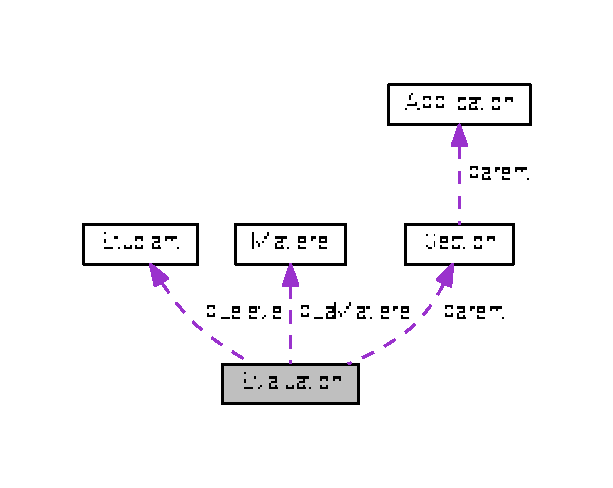
\includegraphics[width=294pt]{class_evaluation__coll__graph}
\end{center}
\end{figure}
\subsection*{Public Member Functions}
\begin{DoxyCompactItemize}
\item 
\hyperlink{class_evaluation_afeed6d48b3009cfadb5d56acacd5af31}{Evaluation} (\hyperlink{class_section}{Section} $\ast$lien)
\item 
void \hyperlink{class_evaluation_a9f6db9e9282e6d1ecd00785db0538b4d}{input\+Evaluation} ()
\item 
void \hyperlink{class_evaluation_ab7114383e258c7d0c8b5e465e0939663}{display\+Evaluation} ()
\end{DoxyCompactItemize}
\subsection*{Private Attributes}
\begin{DoxyCompactItemize}
\item 
\hyperlink{class_section}{Section} $\ast$ \hyperlink{class_evaluation_a5d6336cee965270904fe3d91c6d484a1}{parent}
\item 
\hyperlink{class_matiere}{Matiere} $\ast$ \hyperlink{class_evaluation_ad5f4d301c80076389e2ea31dfd7f09b1}{p\+La\+Matiere}
\item 
\hyperlink{class_etudiant}{Etudiant} $\ast$ \hyperlink{class_evaluation_a38afbf18ba9d4cd79055807d13c88c9f}{p\+Leleve}
\item 
int \hyperlink{class_evaluation_ae000ec143562ed56975018bf82b13b5c}{semestre}
\item 
vector$<$ \hyperlink{class_note}{Note} $>$ \hyperlink{class_evaluation_ac3f2543471f61f13fdaab768960f31fc}{vect\+Notes}
\item 
string \hyperlink{class_evaluation_a3babca319a639a0f4811158cbbc47eb9}{nom\+Eval}
\end{DoxyCompactItemize}


\subsection{Detailed Description}
Permet de créer et d'interagir avec des évaluations. 

\subsection{Constructor \& Destructor Documentation}
\hypertarget{class_evaluation_afeed6d48b3009cfadb5d56acacd5af31}{\index{Evaluation@{Evaluation}!Evaluation@{Evaluation}}
\index{Evaluation@{Evaluation}!Evaluation@{Evaluation}}
\subsubsection[{Evaluation}]{\setlength{\rightskip}{0pt plus 5cm}Evaluation\+::\+Evaluation (
\begin{DoxyParamCaption}
\item[{{\bf Section} $\ast$}]{lien}
\end{DoxyParamCaption}
)}}\label{class_evaluation_afeed6d48b3009cfadb5d56acacd5af31}


\subsection{Member Function Documentation}
\hypertarget{class_evaluation_ab7114383e258c7d0c8b5e465e0939663}{\index{Evaluation@{Evaluation}!display\+Evaluation@{display\+Evaluation}}
\index{display\+Evaluation@{display\+Evaluation}!Evaluation@{Evaluation}}
\subsubsection[{display\+Evaluation}]{\setlength{\rightskip}{0pt plus 5cm}void Evaluation\+::display\+Evaluation (
\begin{DoxyParamCaption}
{}
\end{DoxyParamCaption}
)}}\label{class_evaluation_ab7114383e258c7d0c8b5e465e0939663}
\hypertarget{class_evaluation_a9f6db9e9282e6d1ecd00785db0538b4d}{\index{Evaluation@{Evaluation}!input\+Evaluation@{input\+Evaluation}}
\index{input\+Evaluation@{input\+Evaluation}!Evaluation@{Evaluation}}
\subsubsection[{input\+Evaluation}]{\setlength{\rightskip}{0pt plus 5cm}void Evaluation\+::input\+Evaluation (
\begin{DoxyParamCaption}
{}
\end{DoxyParamCaption}
)}}\label{class_evaluation_a9f6db9e9282e6d1ecd00785db0538b4d}


\subsection{Member Data Documentation}
\hypertarget{class_evaluation_a3babca319a639a0f4811158cbbc47eb9}{\index{Evaluation@{Evaluation}!nom\+Eval@{nom\+Eval}}
\index{nom\+Eval@{nom\+Eval}!Evaluation@{Evaluation}}
\subsubsection[{nom\+Eval}]{\setlength{\rightskip}{0pt plus 5cm}string Evaluation\+::nom\+Eval\hspace{0.3cm}{\ttfamily [private]}}}\label{class_evaluation_a3babca319a639a0f4811158cbbc47eb9}
\hypertarget{class_evaluation_a5d6336cee965270904fe3d91c6d484a1}{\index{Evaluation@{Evaluation}!parent@{parent}}
\index{parent@{parent}!Evaluation@{Evaluation}}
\subsubsection[{parent}]{\setlength{\rightskip}{0pt plus 5cm}{\bf Section}$\ast$ Evaluation\+::parent\hspace{0.3cm}{\ttfamily [private]}}}\label{class_evaluation_a5d6336cee965270904fe3d91c6d484a1}
\hypertarget{class_evaluation_ad5f4d301c80076389e2ea31dfd7f09b1}{\index{Evaluation@{Evaluation}!p\+La\+Matiere@{p\+La\+Matiere}}
\index{p\+La\+Matiere@{p\+La\+Matiere}!Evaluation@{Evaluation}}
\subsubsection[{p\+La\+Matiere}]{\setlength{\rightskip}{0pt plus 5cm}{\bf Matiere}$\ast$ Evaluation\+::p\+La\+Matiere\hspace{0.3cm}{\ttfamily [private]}}}\label{class_evaluation_ad5f4d301c80076389e2ea31dfd7f09b1}
\hypertarget{class_evaluation_a38afbf18ba9d4cd79055807d13c88c9f}{\index{Evaluation@{Evaluation}!p\+Leleve@{p\+Leleve}}
\index{p\+Leleve@{p\+Leleve}!Evaluation@{Evaluation}}
\subsubsection[{p\+Leleve}]{\setlength{\rightskip}{0pt plus 5cm}{\bf Etudiant}$\ast$ Evaluation\+::p\+Leleve\hspace{0.3cm}{\ttfamily [private]}}}\label{class_evaluation_a38afbf18ba9d4cd79055807d13c88c9f}
\hypertarget{class_evaluation_ae000ec143562ed56975018bf82b13b5c}{\index{Evaluation@{Evaluation}!semestre@{semestre}}
\index{semestre@{semestre}!Evaluation@{Evaluation}}
\subsubsection[{semestre}]{\setlength{\rightskip}{0pt plus 5cm}int Evaluation\+::semestre\hspace{0.3cm}{\ttfamily [private]}}}\label{class_evaluation_ae000ec143562ed56975018bf82b13b5c}
\hypertarget{class_evaluation_ac3f2543471f61f13fdaab768960f31fc}{\index{Evaluation@{Evaluation}!vect\+Notes@{vect\+Notes}}
\index{vect\+Notes@{vect\+Notes}!Evaluation@{Evaluation}}
\subsubsection[{vect\+Notes}]{\setlength{\rightskip}{0pt plus 5cm}vector$<${\bf Note}$>$ Evaluation\+::vect\+Notes\hspace{0.3cm}{\ttfamily [private]}}}\label{class_evaluation_ac3f2543471f61f13fdaab768960f31fc}


The documentation for this class was generated from the following file\+:\begin{DoxyCompactItemize}
\item 
\hyperlink{evaluation_8h}{evaluation.\+h}\end{DoxyCompactItemize}

\hypertarget{class_matiere}{\section{Matiere Class Reference}
\label{class_matiere}\index{Matiere@{Matiere}}
}


Permet de créer et d'interagir avec les matières.  




{\ttfamily \#include $<$matiere.\+h$>$}

\subsection*{Public Member Functions}
\begin{DoxyCompactItemize}
\item 
\hyperlink{class_matiere_a0d9dbc35cd0221225366e2ba189c4b42}{Matiere} ()
\item 
\hyperlink{class_matiere_a3a44d93c8078dc274999e7017b27075b}{Matiere} (string nom\+De\+La\+Matiere)
\item 
void \hyperlink{class_matiere_a314ae9fc824027e032c9c02faf3ccc8f}{input} ()
\item 
void \hyperlink{class_matiere_a83c7ad70642d1c15c2b43c5e6c2823d2}{display} ()
\item 
void \hyperlink{class_matiere_a270e13c81b9ad19c42c2128f983af115}{calcul\+Moyenne} ()
\item 
string \hyperlink{class_matiere_a5a31f5b5b20f39cdbf6136cde25ecd31}{get\+Nom\+Matiere} ()
\end{DoxyCompactItemize}
\subsection*{Private Attributes}
\begin{DoxyCompactItemize}
\item 
string \hyperlink{class_matiere_a701728c9283e82fd270a91a8eb541917}{nom\+Matiere}
\end{DoxyCompactItemize}


\subsection{Detailed Description}
Permet de créer et d'interagir avec les matières. 

\subsection{Constructor \& Destructor Documentation}
\hypertarget{class_matiere_a0d9dbc35cd0221225366e2ba189c4b42}{\index{Matiere@{Matiere}!Matiere@{Matiere}}
\index{Matiere@{Matiere}!Matiere@{Matiere}}
\subsubsection[{Matiere}]{\setlength{\rightskip}{0pt plus 5cm}Matiere\+::\+Matiere (
\begin{DoxyParamCaption}
{}
\end{DoxyParamCaption}
)}}\label{class_matiere_a0d9dbc35cd0221225366e2ba189c4b42}
\hypertarget{class_matiere_a3a44d93c8078dc274999e7017b27075b}{\index{Matiere@{Matiere}!Matiere@{Matiere}}
\index{Matiere@{Matiere}!Matiere@{Matiere}}
\subsubsection[{Matiere}]{\setlength{\rightskip}{0pt plus 5cm}Matiere\+::\+Matiere (
\begin{DoxyParamCaption}
\item[{string}]{nom\+De\+La\+Matiere}
\end{DoxyParamCaption}
)}}\label{class_matiere_a3a44d93c8078dc274999e7017b27075b}


\subsection{Member Function Documentation}
\hypertarget{class_matiere_a270e13c81b9ad19c42c2128f983af115}{\index{Matiere@{Matiere}!calcul\+Moyenne@{calcul\+Moyenne}}
\index{calcul\+Moyenne@{calcul\+Moyenne}!Matiere@{Matiere}}
\subsubsection[{calcul\+Moyenne}]{\setlength{\rightskip}{0pt plus 5cm}void Matiere\+::calcul\+Moyenne (
\begin{DoxyParamCaption}
{}
\end{DoxyParamCaption}
)}}\label{class_matiere_a270e13c81b9ad19c42c2128f983af115}
\hypertarget{class_matiere_a83c7ad70642d1c15c2b43c5e6c2823d2}{\index{Matiere@{Matiere}!display@{display}}
\index{display@{display}!Matiere@{Matiere}}
\subsubsection[{display}]{\setlength{\rightskip}{0pt plus 5cm}void Matiere\+::display (
\begin{DoxyParamCaption}
{}
\end{DoxyParamCaption}
)}}\label{class_matiere_a83c7ad70642d1c15c2b43c5e6c2823d2}
\hypertarget{class_matiere_a5a31f5b5b20f39cdbf6136cde25ecd31}{\index{Matiere@{Matiere}!get\+Nom\+Matiere@{get\+Nom\+Matiere}}
\index{get\+Nom\+Matiere@{get\+Nom\+Matiere}!Matiere@{Matiere}}
\subsubsection[{get\+Nom\+Matiere}]{\setlength{\rightskip}{0pt plus 5cm}string Matiere\+::get\+Nom\+Matiere (
\begin{DoxyParamCaption}
{}
\end{DoxyParamCaption}
)}}\label{class_matiere_a5a31f5b5b20f39cdbf6136cde25ecd31}
\hypertarget{class_matiere_a314ae9fc824027e032c9c02faf3ccc8f}{\index{Matiere@{Matiere}!input@{input}}
\index{input@{input}!Matiere@{Matiere}}
\subsubsection[{input}]{\setlength{\rightskip}{0pt plus 5cm}void Matiere\+::input (
\begin{DoxyParamCaption}
{}
\end{DoxyParamCaption}
)}}\label{class_matiere_a314ae9fc824027e032c9c02faf3ccc8f}


\subsection{Member Data Documentation}
\hypertarget{class_matiere_a701728c9283e82fd270a91a8eb541917}{\index{Matiere@{Matiere}!nom\+Matiere@{nom\+Matiere}}
\index{nom\+Matiere@{nom\+Matiere}!Matiere@{Matiere}}
\subsubsection[{nom\+Matiere}]{\setlength{\rightskip}{0pt plus 5cm}string Matiere\+::nom\+Matiere\hspace{0.3cm}{\ttfamily [private]}}}\label{class_matiere_a701728c9283e82fd270a91a8eb541917}


The documentation for this class was generated from the following file\+:\begin{DoxyCompactItemize}
\item 
\hyperlink{matiere_8h}{matiere.\+h}\end{DoxyCompactItemize}

\hypertarget{class_note}{\section{Note Class Reference}
\label{class_note}\index{Note@{Note}}
}


Permet de créer des notes en les lien avec les étudiants.  




{\ttfamily \#include $<$note.\+h$>$}



Collaboration diagram for Note\+:
\nopagebreak
\begin{figure}[H]
\begin{center}
\leavevmode
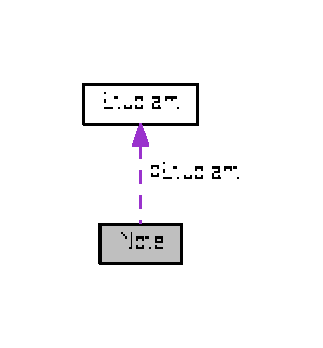
\includegraphics[width=155pt]{class_note__coll__graph}
\end{center}
\end{figure}
\subsection*{Public Member Functions}
\begin{DoxyCompactItemize}
\item 
string \hyperlink{class_note_a48a8448ab0710a4445897d05a31c1efa}{get\+Note} ()
\item 
void \hyperlink{class_note_a0051b1bf8ab17897dcad83ba3e07e456}{set\+Note} (int note\+Entree)
\item 
void \hyperlink{class_note_a2232542d07b8c3657c0e43da23afaedf}{input\+Note} ()
\end{DoxyCompactItemize}
\subsection*{Private Attributes}
\begin{DoxyCompactItemize}
\item 
int \hyperlink{class_note_a3cb5f22dd5374f4e3c59c5f11dc7fbfb}{note}
\item 
\hyperlink{class_etudiant}{Etudiant} $\ast$ \hyperlink{class_note_a3ceec90c97d49215fe0eaa33e92a83d2}{p\+Etudiant}
\end{DoxyCompactItemize}


\subsection{Detailed Description}
Permet de créer des notes en les lien avec les étudiants. 

\subsection{Member Function Documentation}
\hypertarget{class_note_a48a8448ab0710a4445897d05a31c1efa}{\index{Note@{Note}!get\+Note@{get\+Note}}
\index{get\+Note@{get\+Note}!Note@{Note}}
\subsubsection[{get\+Note}]{\setlength{\rightskip}{0pt plus 5cm}string Note\+::get\+Note (
\begin{DoxyParamCaption}
{}
\end{DoxyParamCaption}
)}}\label{class_note_a48a8448ab0710a4445897d05a31c1efa}
\hypertarget{class_note_a2232542d07b8c3657c0e43da23afaedf}{\index{Note@{Note}!input\+Note@{input\+Note}}
\index{input\+Note@{input\+Note}!Note@{Note}}
\subsubsection[{input\+Note}]{\setlength{\rightskip}{0pt plus 5cm}void Note\+::input\+Note (
\begin{DoxyParamCaption}
{}
\end{DoxyParamCaption}
)}}\label{class_note_a2232542d07b8c3657c0e43da23afaedf}
\hypertarget{class_note_a0051b1bf8ab17897dcad83ba3e07e456}{\index{Note@{Note}!set\+Note@{set\+Note}}
\index{set\+Note@{set\+Note}!Note@{Note}}
\subsubsection[{set\+Note}]{\setlength{\rightskip}{0pt plus 5cm}void Note\+::set\+Note (
\begin{DoxyParamCaption}
\item[{int}]{note\+Entree}
\end{DoxyParamCaption}
)}}\label{class_note_a0051b1bf8ab17897dcad83ba3e07e456}


\subsection{Member Data Documentation}
\hypertarget{class_note_a3cb5f22dd5374f4e3c59c5f11dc7fbfb}{\index{Note@{Note}!note@{note}}
\index{note@{note}!Note@{Note}}
\subsubsection[{note}]{\setlength{\rightskip}{0pt plus 5cm}int Note\+::note\hspace{0.3cm}{\ttfamily [private]}}}\label{class_note_a3cb5f22dd5374f4e3c59c5f11dc7fbfb}
\hypertarget{class_note_a3ceec90c97d49215fe0eaa33e92a83d2}{\index{Note@{Note}!p\+Etudiant@{p\+Etudiant}}
\index{p\+Etudiant@{p\+Etudiant}!Note@{Note}}
\subsubsection[{p\+Etudiant}]{\setlength{\rightskip}{0pt plus 5cm}{\bf Etudiant}$\ast$ Note\+::p\+Etudiant\hspace{0.3cm}{\ttfamily [private]}}}\label{class_note_a3ceec90c97d49215fe0eaa33e92a83d2}


The documentation for this class was generated from the following file\+:\begin{DoxyCompactItemize}
\item 
\hyperlink{note_8h}{note.\+h}\end{DoxyCompactItemize}

\hypertarget{class_section}{\section{Section Class Reference}
\label{class_section}\index{Section@{Section}}
}


Permet le liens avec \hyperlink{class_section}{Section} pour en utiliser des éléments.  




{\ttfamily \#include $<$section.\+h$>$}



Collaboration diagram for Section\+:
\nopagebreak
\begin{figure}[H]
\begin{center}
\leavevmode
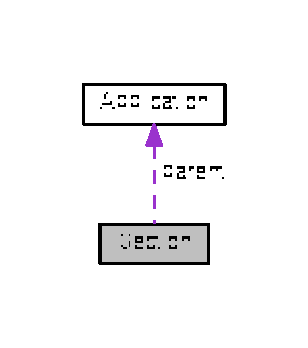
\includegraphics[width=148pt]{class_section__coll__graph}
\end{center}
\end{figure}
\subsection*{Public Member Functions}
\begin{DoxyCompactItemize}
\item 
vector$<$ \hyperlink{class_matiere}{Matiere} $\ast$ $>$ \hyperlink{class_section_a7d11b3ccad35aea44d0e2b0ab9697e94}{get\+Vect\+Matiere} ()
\begin{DoxyCompactList}\small\item\em Méthodes utilisée par \hyperlink{class_section}{Section} pour récupérer toutes les matières de \hyperlink{class_application}{Application}. \end{DoxyCompactList}\item 
vector$<$ \hyperlink{class_etudiant}{Etudiant} $>$ $\ast$ \hyperlink{class_section_a91998036826e5c3fd63baee29f61af56}{get\+Vect\+Eleve} ()
\begin{DoxyCompactList}\small\item\em Méthode utilisée par \hyperlink{class_section}{Section} pour récupérer tous les élève de \hyperlink{class_section}{Section}. \end{DoxyCompactList}\item 
\hyperlink{class_section_a4e65b11fb3fa5fba337053389bedbfe5}{Section} (\hyperlink{class_application}{Application} $\ast$lien)
\begin{DoxyCompactList}\small\item\em Constructeur d'un lien permettant de récupérer des éléments d'\hyperlink{class_application}{Application} (notament les matières) \end{DoxyCompactList}\item 
\hyperlink{class_section_aefbd9080252dec03fa54bcf06d669956}{Section} (string nom\+De\+La\+Section, \hyperlink{class_application}{Application} $\ast$lien)
\begin{DoxyCompactList}\small\item\em Constructeur d'une section étant dans application (Création de jeu d'essai) \end{DoxyCompactList}\item 
void \hyperlink{class_section_a1f9ebccdb1937ca61a0d4adcde310832}{display} ()
\begin{DoxyCompactList}\small\item\em utilisée par Seciton, affiche le contenu de section \end{DoxyCompactList}\item 
void \hyperlink{class_section_a32e3a0a0682f01437a82ddbf7dd59b0a}{input} ()
\begin{DoxyCompactList}\small\item\em utilisé par \hyperlink{class_section}{Section}, demande la saisie des informations d'un \hyperlink{class_section}{Section} (son nom) \end{DoxyCompactList}\item 
string \hyperlink{class_section_a432b7a6163aa6225e74de5560fe09b00}{get\+Nom\+Section} ()
\begin{DoxyCompactList}\small\item\em utilisée par \hyperlink{class_section}{Section} accède au nom de la section \end{DoxyCompactList}\item 
void \hyperlink{class_section_aaa255f02935c89189d64037ec453495b}{set\+Nom\+Section} (string \hyperlink{class_section_a74c53e192d8055ffe2ef8ca0e814662c}{nomsection})
\begin{DoxyCompactList}\small\item\em utilisée par \hyperlink{class_section}{Section}, permet de modifier le nom de la seciton \end{DoxyCompactList}\item 
void \hyperlink{class_section_a22fe3717cd11f7192f39c71c9131b24f}{affichage\+Toute\+Matieres\+App} ()
\begin{DoxyCompactList}\small\item\em utilisée par \hyperlink{class_section}{Section}, affiche toutes les matières de l'\hyperlink{class_application}{Application} \end{DoxyCompactList}\item 
void \hyperlink{class_section_a6334f5782c68c7bfc076f9c3a4e3ef50}{afficher\+Eleves} ()
\begin{DoxyCompactList}\small\item\em utilisée par \hyperlink{class_section}{Section}, affiche tous les élève de la section dans laquelle on est \end{DoxyCompactList}\item 
void \hyperlink{class_section_afa8816db504195a8c1f5c9d8c3ccbd34}{ajouter\+Eleve} ()
\begin{DoxyCompactList}\small\item\em utilisée par \hyperlink{class_section}{Section}, permet d'y ajouter un élève \end{DoxyCompactList}\item 
void \hyperlink{class_section_a9ccb8ae4950c3fb7003283d63eeb1f2a}{afficher\+Evaluations} ()
\begin{DoxyCompactList}\small\item\em utilisée par \hyperlink{class_section}{Section}, permet d'afficher les notes de chaque élève a une évaluation (to end) \end{DoxyCompactList}\item 
void \hyperlink{class_section_a7ca7b4088ad4326533a300581ac6f6a0}{ajouter\+Evaluation} ()
\begin{DoxyCompactList}\small\item\em utilisée par \hyperlink{class_section}{Section}, permet d'ajouter une évaluation = une note a chaque élève, une matière et une date(semestre) \end{DoxyCompactList}\item 
void \hyperlink{class_section_aad00712e76a9116295cd48ca475e4289}{afficher\+Matieres} ()
\begin{DoxyCompactList}\small\item\em utilisée par \hyperlink{class_section}{Section}, permet d'afficher les matière de la section \end{DoxyCompactList}\item 
void \hyperlink{class_section_af834dd53f188641f0b1cc24d7d18e919}{ajouter\+Matiere} ()
\begin{DoxyCompactList}\small\item\em utilisée par \hyperlink{class_section}{Section}, permet d'ajouter une matière a la secion parmis celle d'\hyperlink{class_application}{Application} \end{DoxyCompactList}\item 
void \hyperlink{class_section_a27cba40cc111707559dce0dfd4c5bf61}{run\+Section} ()
\begin{DoxyCompactList}\small\item\em utilisée par \hyperlink{class_application}{Application}, permet de lancer les interactions avec une section séléctionné dans \hyperlink{class_application}{Application} \end{DoxyCompactList}\item 
void \hyperlink{class_section_a37f98cee5c7b99d30d29cc829a541ea6}{Afficher\+Menu\+Section} ()
\begin{DoxyCompactList}\small\item\em utilisée par \hyperlink{class_section}{Section}, affiche le menu principale de \hyperlink{class_section}{Section} \end{DoxyCompactList}\item 
char \hyperlink{class_section_a1bff0e887b4858183de5baf404922989}{saisie\+Controle\+Du\+Choix\+Utilisateur} ()
\begin{DoxyCompactList}\small\item\em Permet de connaitre le choix de l'utilisateur afin d'éxécuter l'aciton demandée. \end{DoxyCompactList}\item 
void \hyperlink{class_section_aa17b8729ea8bac8a936c2a34a03a06a2}{realisation\+Action\+Correspondante\+Au\+Choix} (char le\+Choix)
\begin{DoxyCompactList}\small\item\em Exécute l'action choisi par l'utilisateur. \end{DoxyCompactList}\end{DoxyCompactItemize}
\subsection*{Private Attributes}
\begin{DoxyCompactItemize}
\item 
string \hyperlink{class_section_a74c53e192d8055ffe2ef8ca0e814662c}{nomsection}
\begin{DoxyCompactList}\small\item\em Nom de la section. \end{DoxyCompactList}\item 
vector$<$ \hyperlink{class_etudiant}{Etudiant} $>$ \hyperlink{class_section_a53c0f63296e6c0a58208f3f13b6eb1a0}{vect\+Eleve}
\begin{DoxyCompactList}\small\item\em vecteur d'élève propre a \hyperlink{class_section}{Section} \end{DoxyCompactList}\item 
vector$<$ \hyperlink{class_evaluation}{Evaluation} $>$ \hyperlink{class_section_ad1006e87bbe4c2ac441c12504cc16fa4}{vect\+Eval}
\begin{DoxyCompactList}\small\item\em vecteur d'évaluation propre a \hyperlink{class_section}{Section} \end{DoxyCompactList}\item 
vector$<$ \hyperlink{class_matiere}{Matiere} $\ast$ $>$ \hyperlink{class_section_ab4d854da53a93ae314bef4f849ab7649}{vect\+Matiere}
\begin{DoxyCompactList}\small\item\em vecteur de pointeur de Matière d'\hyperlink{class_application}{Application} (parti des matière propre a une \hyperlink{class_section}{Section}) \end{DoxyCompactList}\item 
vector$<$ int $>$ \hyperlink{class_section_a804c0479bba4cb92a12823c10e1e6944}{vect\+Coeff}
\begin{DoxyCompactList}\small\item\em vecteur de coefficient des matière de la \hyperlink{class_section}{Section} (ex\+: Maths est Coef 7 pour la \hyperlink{class_section}{Section} Terminal S1) \end{DoxyCompactList}\item 
\hyperlink{class_application}{Application} $\ast$ \hyperlink{class_section_af3bb36866f8d63e6059ba7b54247eb7c}{parent}
\begin{DoxyCompactList}\small\item\em Pointeur d'applicaion permettant le lien entre \hyperlink{class_section}{Section} et \hyperlink{class_application}{Application} (pour en récupérer les matiere notament) \end{DoxyCompactList}\end{DoxyCompactItemize}


\subsection{Detailed Description}
Permet le liens avec \hyperlink{class_section}{Section} pour en utiliser des éléments. 

Ensemble des interactions ente l'utilisateur et les sections. 

\subsection{Constructor \& Destructor Documentation}
\hypertarget{class_section_a4e65b11fb3fa5fba337053389bedbfe5}{\index{Section@{Section}!Section@{Section}}
\index{Section@{Section}!Section@{Section}}
\subsubsection[{Section}]{\setlength{\rightskip}{0pt plus 5cm}Section\+::\+Section (
\begin{DoxyParamCaption}
\item[{{\bf Application} $\ast$}]{lien}
\end{DoxyParamCaption}
)}}\label{class_section_a4e65b11fb3fa5fba337053389bedbfe5}


Constructeur d'un lien permettant de récupérer des éléments d'\hyperlink{class_application}{Application} (notament les matières) 


\begin{DoxyParams}{Parameters}
{\em adresse} & d'\hyperlink{class_application}{Application} \\
\hline
\end{DoxyParams}
\begin{DoxyReturn}{Returns}
une \hyperlink{class_section}{Section} 
\end{DoxyReturn}
\hypertarget{class_section_aefbd9080252dec03fa54bcf06d669956}{\index{Section@{Section}!Section@{Section}}
\index{Section@{Section}!Section@{Section}}
\subsubsection[{Section}]{\setlength{\rightskip}{0pt plus 5cm}Section\+::\+Section (
\begin{DoxyParamCaption}
\item[{string}]{nom\+De\+La\+Section, }
\item[{{\bf Application} $\ast$}]{lien}
\end{DoxyParamCaption}
)}}\label{class_section_aefbd9080252dec03fa54bcf06d669956}


Constructeur d'une section étant dans application (Création de jeu d'essai) 


\begin{DoxyParams}{Parameters}
{\em un} & nom de section et une adresse vers \hyperlink{class_application}{Application} \\
\hline
\end{DoxyParams}
\begin{DoxyReturn}{Returns}
une \hyperlink{class_section}{Section} 
\end{DoxyReturn}


\subsection{Member Function Documentation}
\hypertarget{class_section_a22fe3717cd11f7192f39c71c9131b24f}{\index{Section@{Section}!affichage\+Toute\+Matieres\+App@{affichage\+Toute\+Matieres\+App}}
\index{affichage\+Toute\+Matieres\+App@{affichage\+Toute\+Matieres\+App}!Section@{Section}}
\subsubsection[{affichage\+Toute\+Matieres\+App}]{\setlength{\rightskip}{0pt plus 5cm}void Section\+::affichage\+Toute\+Matieres\+App (
\begin{DoxyParamCaption}
{}
\end{DoxyParamCaption}
)}}\label{class_section_a22fe3717cd11f7192f39c71c9131b24f}


utilisée par \hyperlink{class_section}{Section}, affiche toutes les matières de l'\hyperlink{class_application}{Application} 

\hypertarget{class_section_a6334f5782c68c7bfc076f9c3a4e3ef50}{\index{Section@{Section}!afficher\+Eleves@{afficher\+Eleves}}
\index{afficher\+Eleves@{afficher\+Eleves}!Section@{Section}}
\subsubsection[{afficher\+Eleves}]{\setlength{\rightskip}{0pt plus 5cm}void Section\+::afficher\+Eleves (
\begin{DoxyParamCaption}
{}
\end{DoxyParamCaption}
)}}\label{class_section_a6334f5782c68c7bfc076f9c3a4e3ef50}


utilisée par \hyperlink{class_section}{Section}, affiche tous les élève de la section dans laquelle on est 

\hypertarget{class_section_a9ccb8ae4950c3fb7003283d63eeb1f2a}{\index{Section@{Section}!afficher\+Evaluations@{afficher\+Evaluations}}
\index{afficher\+Evaluations@{afficher\+Evaluations}!Section@{Section}}
\subsubsection[{afficher\+Evaluations}]{\setlength{\rightskip}{0pt plus 5cm}void Section\+::afficher\+Evaluations (
\begin{DoxyParamCaption}
{}
\end{DoxyParamCaption}
)}}\label{class_section_a9ccb8ae4950c3fb7003283d63eeb1f2a}


utilisée par \hyperlink{class_section}{Section}, permet d'afficher les notes de chaque élève a une évaluation (to end) 

\hypertarget{class_section_aad00712e76a9116295cd48ca475e4289}{\index{Section@{Section}!afficher\+Matieres@{afficher\+Matieres}}
\index{afficher\+Matieres@{afficher\+Matieres}!Section@{Section}}
\subsubsection[{afficher\+Matieres}]{\setlength{\rightskip}{0pt plus 5cm}void Section\+::afficher\+Matieres (
\begin{DoxyParamCaption}
{}
\end{DoxyParamCaption}
)}}\label{class_section_aad00712e76a9116295cd48ca475e4289}


utilisée par \hyperlink{class_section}{Section}, permet d'afficher les matière de la section 

\hypertarget{class_section_a37f98cee5c7b99d30d29cc829a541ea6}{\index{Section@{Section}!Afficher\+Menu\+Section@{Afficher\+Menu\+Section}}
\index{Afficher\+Menu\+Section@{Afficher\+Menu\+Section}!Section@{Section}}
\subsubsection[{Afficher\+Menu\+Section}]{\setlength{\rightskip}{0pt plus 5cm}void Section\+::\+Afficher\+Menu\+Section (
\begin{DoxyParamCaption}
{}
\end{DoxyParamCaption}
)}}\label{class_section_a37f98cee5c7b99d30d29cc829a541ea6}


utilisée par \hyperlink{class_section}{Section}, affiche le menu principale de \hyperlink{class_section}{Section} 

\hypertarget{class_section_afa8816db504195a8c1f5c9d8c3ccbd34}{\index{Section@{Section}!ajouter\+Eleve@{ajouter\+Eleve}}
\index{ajouter\+Eleve@{ajouter\+Eleve}!Section@{Section}}
\subsubsection[{ajouter\+Eleve}]{\setlength{\rightskip}{0pt plus 5cm}void Section\+::ajouter\+Eleve (
\begin{DoxyParamCaption}
{}
\end{DoxyParamCaption}
)}}\label{class_section_afa8816db504195a8c1f5c9d8c3ccbd34}


utilisée par \hyperlink{class_section}{Section}, permet d'y ajouter un élève 

\hypertarget{class_section_a7ca7b4088ad4326533a300581ac6f6a0}{\index{Section@{Section}!ajouter\+Evaluation@{ajouter\+Evaluation}}
\index{ajouter\+Evaluation@{ajouter\+Evaluation}!Section@{Section}}
\subsubsection[{ajouter\+Evaluation}]{\setlength{\rightskip}{0pt plus 5cm}void Section\+::ajouter\+Evaluation (
\begin{DoxyParamCaption}
{}
\end{DoxyParamCaption}
)}}\label{class_section_a7ca7b4088ad4326533a300581ac6f6a0}


utilisée par \hyperlink{class_section}{Section}, permet d'ajouter une évaluation = une note a chaque élève, une matière et une date(semestre) 

\hypertarget{class_section_af834dd53f188641f0b1cc24d7d18e919}{\index{Section@{Section}!ajouter\+Matiere@{ajouter\+Matiere}}
\index{ajouter\+Matiere@{ajouter\+Matiere}!Section@{Section}}
\subsubsection[{ajouter\+Matiere}]{\setlength{\rightskip}{0pt plus 5cm}void Section\+::ajouter\+Matiere (
\begin{DoxyParamCaption}
{}
\end{DoxyParamCaption}
)}}\label{class_section_af834dd53f188641f0b1cc24d7d18e919}


utilisée par \hyperlink{class_section}{Section}, permet d'ajouter une matière a la secion parmis celle d'\hyperlink{class_application}{Application} 

\hypertarget{class_section_a1f9ebccdb1937ca61a0d4adcde310832}{\index{Section@{Section}!display@{display}}
\index{display@{display}!Section@{Section}}
\subsubsection[{display}]{\setlength{\rightskip}{0pt plus 5cm}void Section\+::display (
\begin{DoxyParamCaption}
{}
\end{DoxyParamCaption}
)}}\label{class_section_a1f9ebccdb1937ca61a0d4adcde310832}


utilisée par Seciton, affiche le contenu de section 

\hypertarget{class_section_a432b7a6163aa6225e74de5560fe09b00}{\index{Section@{Section}!get\+Nom\+Section@{get\+Nom\+Section}}
\index{get\+Nom\+Section@{get\+Nom\+Section}!Section@{Section}}
\subsubsection[{get\+Nom\+Section}]{\setlength{\rightskip}{0pt plus 5cm}string Section\+::get\+Nom\+Section (
\begin{DoxyParamCaption}
{}
\end{DoxyParamCaption}
)}}\label{class_section_a432b7a6163aa6225e74de5560fe09b00}


utilisée par \hyperlink{class_section}{Section} accède au nom de la section 

return string du nom de la section \hypertarget{class_section_a91998036826e5c3fd63baee29f61af56}{\index{Section@{Section}!get\+Vect\+Eleve@{get\+Vect\+Eleve}}
\index{get\+Vect\+Eleve@{get\+Vect\+Eleve}!Section@{Section}}
\subsubsection[{get\+Vect\+Eleve}]{\setlength{\rightskip}{0pt plus 5cm}vector$<$ {\bf Etudiant} $>$ $\ast$ Section\+::get\+Vect\+Eleve (
\begin{DoxyParamCaption}
{}
\end{DoxyParamCaption}
)}}\label{class_section_a91998036826e5c3fd63baee29f61af56}


Méthode utilisée par \hyperlink{class_section}{Section} pour récupérer tous les élève de \hyperlink{class_section}{Section}. 

\begin{DoxyReturn}{Returns}
un vecteur pointeur d'Etudiants de la \hyperlink{class_section}{Section} 
\end{DoxyReturn}
\hypertarget{class_section_a7d11b3ccad35aea44d0e2b0ab9697e94}{\index{Section@{Section}!get\+Vect\+Matiere@{get\+Vect\+Matiere}}
\index{get\+Vect\+Matiere@{get\+Vect\+Matiere}!Section@{Section}}
\subsubsection[{get\+Vect\+Matiere}]{\setlength{\rightskip}{0pt plus 5cm}vector$<$ {\bf Matiere} $\ast$ $>$ Section\+::get\+Vect\+Matiere (
\begin{DoxyParamCaption}
{}
\end{DoxyParamCaption}
)}}\label{class_section_a7d11b3ccad35aea44d0e2b0ab9697e94}


Méthodes utilisée par \hyperlink{class_section}{Section} pour récupérer toutes les matières de \hyperlink{class_application}{Application}. 

\begin{DoxyReturn}{Returns}
un vecteur de pointeur de \hyperlink{class_matiere}{Matiere} d'\hyperlink{class_application}{Application} 
\end{DoxyReturn}
\hypertarget{class_section_a32e3a0a0682f01437a82ddbf7dd59b0a}{\index{Section@{Section}!input@{input}}
\index{input@{input}!Section@{Section}}
\subsubsection[{input}]{\setlength{\rightskip}{0pt plus 5cm}void Section\+::input (
\begin{DoxyParamCaption}
{}
\end{DoxyParamCaption}
)}}\label{class_section_a32e3a0a0682f01437a82ddbf7dd59b0a}


utilisé par \hyperlink{class_section}{Section}, demande la saisie des informations d'un \hyperlink{class_section}{Section} (son nom) 

\hypertarget{class_section_aa17b8729ea8bac8a936c2a34a03a06a2}{\index{Section@{Section}!realisation\+Action\+Correspondante\+Au\+Choix@{realisation\+Action\+Correspondante\+Au\+Choix}}
\index{realisation\+Action\+Correspondante\+Au\+Choix@{realisation\+Action\+Correspondante\+Au\+Choix}!Section@{Section}}
\subsubsection[{realisation\+Action\+Correspondante\+Au\+Choix}]{\setlength{\rightskip}{0pt plus 5cm}void Section\+::realisation\+Action\+Correspondante\+Au\+Choix (
\begin{DoxyParamCaption}
\item[{char}]{le\+Choix}
\end{DoxyParamCaption}
)}}\label{class_section_aa17b8729ea8bac8a936c2a34a03a06a2}


Exécute l'action choisi par l'utilisateur. 

\hypertarget{class_section_a27cba40cc111707559dce0dfd4c5bf61}{\index{Section@{Section}!run\+Section@{run\+Section}}
\index{run\+Section@{run\+Section}!Section@{Section}}
\subsubsection[{run\+Section}]{\setlength{\rightskip}{0pt plus 5cm}void Section\+::run\+Section (
\begin{DoxyParamCaption}
{}
\end{DoxyParamCaption}
)}}\label{class_section_a27cba40cc111707559dce0dfd4c5bf61}


utilisée par \hyperlink{class_application}{Application}, permet de lancer les interactions avec une section séléctionné dans \hyperlink{class_application}{Application} 

\hypertarget{class_section_a1bff0e887b4858183de5baf404922989}{\index{Section@{Section}!saisie\+Controle\+Du\+Choix\+Utilisateur@{saisie\+Controle\+Du\+Choix\+Utilisateur}}
\index{saisie\+Controle\+Du\+Choix\+Utilisateur@{saisie\+Controle\+Du\+Choix\+Utilisateur}!Section@{Section}}
\subsubsection[{saisie\+Controle\+Du\+Choix\+Utilisateur}]{\setlength{\rightskip}{0pt plus 5cm}char Section\+::saisie\+Controle\+Du\+Choix\+Utilisateur (
\begin{DoxyParamCaption}
{}
\end{DoxyParamCaption}
)}}\label{class_section_a1bff0e887b4858183de5baf404922989}


Permet de connaitre le choix de l'utilisateur afin d'éxécuter l'aciton demandée. 

\begin{DoxyReturn}{Returns}
char (lettre choisi par l'utilisateur correspondant a son choix) 
\end{DoxyReturn}
\hypertarget{class_section_aaa255f02935c89189d64037ec453495b}{\index{Section@{Section}!set\+Nom\+Section@{set\+Nom\+Section}}
\index{set\+Nom\+Section@{set\+Nom\+Section}!Section@{Section}}
\subsubsection[{set\+Nom\+Section}]{\setlength{\rightskip}{0pt plus 5cm}void Section\+::set\+Nom\+Section (
\begin{DoxyParamCaption}
\item[{string}]{nomsection}
\end{DoxyParamCaption}
)}}\label{class_section_aaa255f02935c89189d64037ec453495b}


utilisée par \hyperlink{class_section}{Section}, permet de modifier le nom de la seciton 


\begin{DoxyParams}{Parameters}
{\em nom} & d'une section (a modifier) \\
\hline
\end{DoxyParams}


\subsection{Member Data Documentation}
\hypertarget{class_section_a74c53e192d8055ffe2ef8ca0e814662c}{\index{Section@{Section}!nomsection@{nomsection}}
\index{nomsection@{nomsection}!Section@{Section}}
\subsubsection[{nomsection}]{\setlength{\rightskip}{0pt plus 5cm}string Section\+::nomsection\hspace{0.3cm}{\ttfamily [private]}}}\label{class_section_a74c53e192d8055ffe2ef8ca0e814662c}


Nom de la section. 

\hypertarget{class_section_af3bb36866f8d63e6059ba7b54247eb7c}{\index{Section@{Section}!parent@{parent}}
\index{parent@{parent}!Section@{Section}}
\subsubsection[{parent}]{\setlength{\rightskip}{0pt plus 5cm}{\bf Application}$\ast$ Section\+::parent\hspace{0.3cm}{\ttfamily [private]}}}\label{class_section_af3bb36866f8d63e6059ba7b54247eb7c}


Pointeur d'applicaion permettant le lien entre \hyperlink{class_section}{Section} et \hyperlink{class_application}{Application} (pour en récupérer les matiere notament) 

\hypertarget{class_section_a804c0479bba4cb92a12823c10e1e6944}{\index{Section@{Section}!vect\+Coeff@{vect\+Coeff}}
\index{vect\+Coeff@{vect\+Coeff}!Section@{Section}}
\subsubsection[{vect\+Coeff}]{\setlength{\rightskip}{0pt plus 5cm}vector$<$int$>$ Section\+::vect\+Coeff\hspace{0.3cm}{\ttfamily [private]}}}\label{class_section_a804c0479bba4cb92a12823c10e1e6944}


vecteur de coefficient des matière de la \hyperlink{class_section}{Section} (ex\+: Maths est Coef 7 pour la \hyperlink{class_section}{Section} Terminal S1) 

\hypertarget{class_section_a53c0f63296e6c0a58208f3f13b6eb1a0}{\index{Section@{Section}!vect\+Eleve@{vect\+Eleve}}
\index{vect\+Eleve@{vect\+Eleve}!Section@{Section}}
\subsubsection[{vect\+Eleve}]{\setlength{\rightskip}{0pt plus 5cm}vector$<${\bf Etudiant}$>$ Section\+::vect\+Eleve\hspace{0.3cm}{\ttfamily [private]}}}\label{class_section_a53c0f63296e6c0a58208f3f13b6eb1a0}


vecteur d'élève propre a \hyperlink{class_section}{Section} 

\hypertarget{class_section_ad1006e87bbe4c2ac441c12504cc16fa4}{\index{Section@{Section}!vect\+Eval@{vect\+Eval}}
\index{vect\+Eval@{vect\+Eval}!Section@{Section}}
\subsubsection[{vect\+Eval}]{\setlength{\rightskip}{0pt plus 5cm}vector$<${\bf Evaluation}$>$ Section\+::vect\+Eval\hspace{0.3cm}{\ttfamily [private]}}}\label{class_section_ad1006e87bbe4c2ac441c12504cc16fa4}


vecteur d'évaluation propre a \hyperlink{class_section}{Section} 

\hypertarget{class_section_ab4d854da53a93ae314bef4f849ab7649}{\index{Section@{Section}!vect\+Matiere@{vect\+Matiere}}
\index{vect\+Matiere@{vect\+Matiere}!Section@{Section}}
\subsubsection[{vect\+Matiere}]{\setlength{\rightskip}{0pt plus 5cm}vector$<${\bf Matiere}$\ast$$>$ Section\+::vect\+Matiere\hspace{0.3cm}{\ttfamily [private]}}}\label{class_section_ab4d854da53a93ae314bef4f849ab7649}


vecteur de pointeur de Matière d'\hyperlink{class_application}{Application} (parti des matière propre a une \hyperlink{class_section}{Section}) 



The documentation for this class was generated from the following file\+:\begin{DoxyCompactItemize}
\item 
\hyperlink{section_8h}{section.\+h}\end{DoxyCompactItemize}

\chapter{File Documentation}
\hypertarget{application_8h}{\section{application.\+h File Reference}
\label{application_8h}\index{application.\+h@{application.\+h}}
}
{\ttfamily \#include $<$iostream$>$}\\*
{\ttfamily \#include $<$vector$>$}\\*
{\ttfamily \#include \char`\"{}section.\+h\char`\"{}}\\*
Include dependency graph for application.\+h\+:
\nopagebreak
\begin{figure}[H]
\begin{center}
\leavevmode
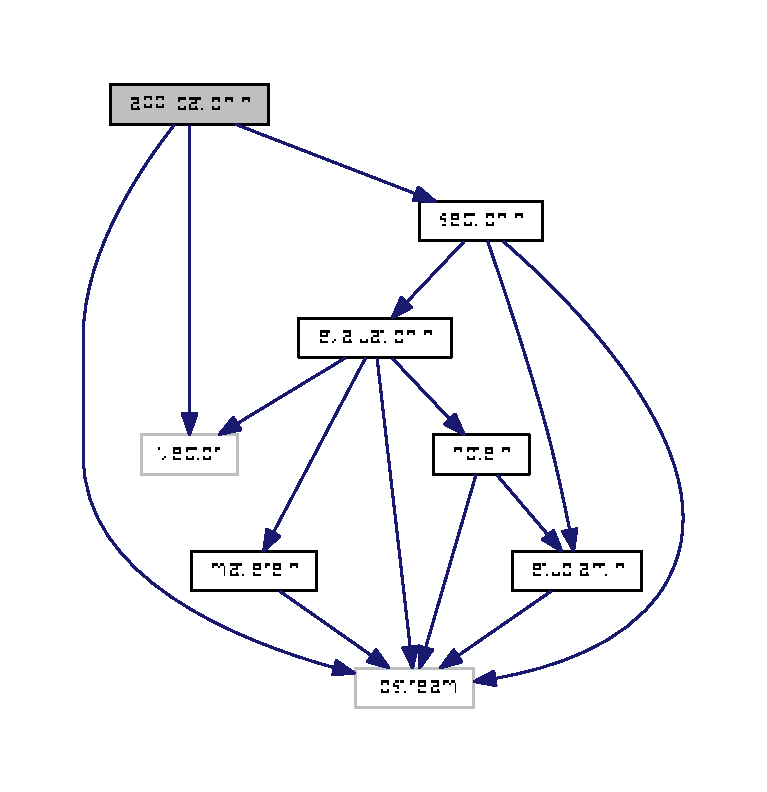
\includegraphics[width=350pt]{application_8h__incl}
\end{center}
\end{figure}
\subsection*{Classes}
\begin{DoxyCompactItemize}
\item 
class \hyperlink{class_application}{Application}
\begin{DoxyCompactList}\small\item\em ensemble des éléments et action du menu principal \end{DoxyCompactList}\end{DoxyCompactItemize}


\subsection{Detailed Description}
\begin{DoxyAuthor}{Author}
Maxime I\+O\+R\+I 
\end{DoxyAuthor}
\begin{DoxyVersion}{Version}
0.\+1 
\end{DoxyVersion}

\hypertarget{bulletin_8h}{\section{bulletin.\+h File Reference}
\label{bulletin_8h}\index{bulletin.\+h@{bulletin.\+h}}
}


\subsection{Detailed Description}
\begin{DoxyAuthor}{Author}
Maxime I\+O\+R\+I 
\end{DoxyAuthor}
\begin{DoxyVersion}{Version}
0.\+1 
\end{DoxyVersion}

\hypertarget{etudiant_8h}{\section{etudiant.\+h File Reference}
\label{etudiant_8h}\index{etudiant.\+h@{etudiant.\+h}}
}
{\ttfamily \#include $<$iostream$>$}\\*
Include dependency graph for etudiant.\+h\+:
\nopagebreak
\begin{figure}[H]
\begin{center}
\leavevmode
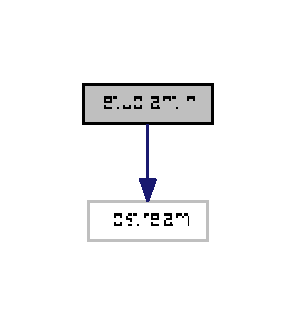
\includegraphics[width=142pt]{etudiant_8h__incl}
\end{center}
\end{figure}
This graph shows which files directly or indirectly include this file\+:
\nopagebreak
\begin{figure}[H]
\begin{center}
\leavevmode
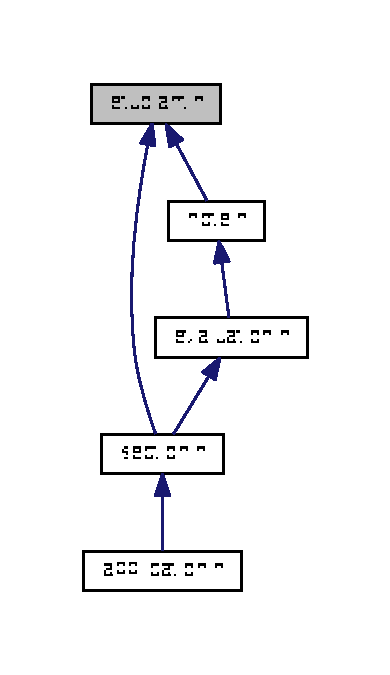
\includegraphics[width=187pt]{etudiant_8h__dep__incl}
\end{center}
\end{figure}
\subsection*{Classes}
\begin{DoxyCompactItemize}
\item 
class \hyperlink{class_etudiant}{Etudiant}
\begin{DoxyCompactList}\small\item\em Permet d'interagir avec les élèves, avoir leurs noms etc... \end{DoxyCompactList}\end{DoxyCompactItemize}


\subsection{Detailed Description}
\begin{DoxyAuthor}{Author}
Maxime I\+O\+R\+I 
\end{DoxyAuthor}
\begin{DoxyVersion}{Version}
0.\+1 
\end{DoxyVersion}

\hypertarget{evaluation_8h}{\section{evaluation.\+h File Reference}
\label{evaluation_8h}\index{evaluation.\+h@{evaluation.\+h}}
}
{\ttfamily \#include $<$iostream$>$}\\*
{\ttfamily \#include $<$vector$>$}\\*
{\ttfamily \#include \char`\"{}note.\+h\char`\"{}}\\*
{\ttfamily \#include \char`\"{}matiere.\+h\char`\"{}}\\*
Include dependency graph for evaluation.\+h\+:
\nopagebreak
\begin{figure}[H]
\begin{center}
\leavevmode
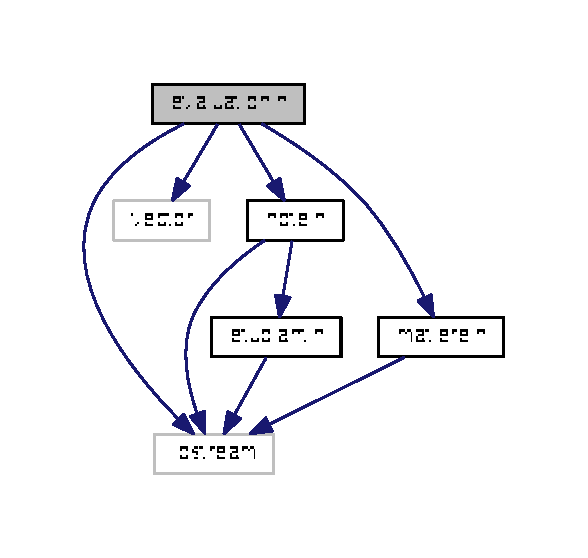
\includegraphics[width=282pt]{evaluation_8h__incl}
\end{center}
\end{figure}
This graph shows which files directly or indirectly include this file\+:
\nopagebreak
\begin{figure}[H]
\begin{center}
\leavevmode
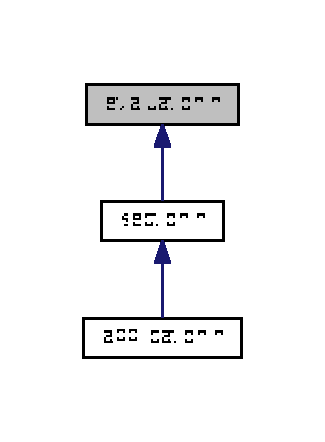
\includegraphics[width=156pt]{evaluation_8h__dep__incl}
\end{center}
\end{figure}
\subsection*{Classes}
\begin{DoxyCompactItemize}
\item 
class \hyperlink{class_evaluation}{Evaluation}
\begin{DoxyCompactList}\small\item\em Permet de créer et d'interagir avec des évaluations. \end{DoxyCompactList}\end{DoxyCompactItemize}


\subsection{Detailed Description}
\begin{DoxyAuthor}{Author}
Maxime I\+O\+R\+I 
\end{DoxyAuthor}
\begin{DoxyVersion}{Version}
0.\+1 
\end{DoxyVersion}

\hypertarget{matiere_8h}{\section{matiere.\+h File Reference}
\label{matiere_8h}\index{matiere.\+h@{matiere.\+h}}
}
{\ttfamily \#include $<$iostream$>$}\\*
Include dependency graph for matiere.\+h\+:
\nopagebreak
\begin{figure}[H]
\begin{center}
\leavevmode
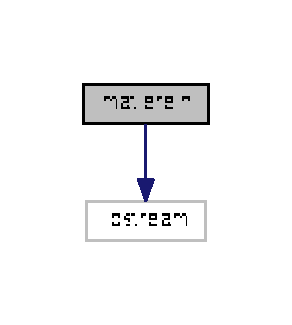
\includegraphics[width=140pt]{matiere_8h__incl}
\end{center}
\end{figure}
This graph shows which files directly or indirectly include this file\+:
\nopagebreak
\begin{figure}[H]
\begin{center}
\leavevmode
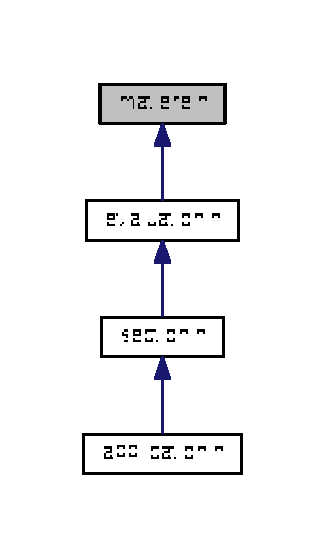
\includegraphics[width=156pt]{matiere_8h__dep__incl}
\end{center}
\end{figure}
\subsection*{Classes}
\begin{DoxyCompactItemize}
\item 
class \hyperlink{class_matiere}{Matiere}
\begin{DoxyCompactList}\small\item\em Permet de créer et d'interagir avec les matières. \end{DoxyCompactList}\end{DoxyCompactItemize}


\subsection{Detailed Description}
\begin{DoxyAuthor}{Author}
Maxime I\+O\+R\+I 
\end{DoxyAuthor}
\begin{DoxyVersion}{Version}
0.\+1 
\end{DoxyVersion}

\hypertarget{note_8h}{\section{note.\+h File Reference}
\label{note_8h}\index{note.\+h@{note.\+h}}
}
{\ttfamily \#include $<$iostream$>$}\\*
{\ttfamily \#include \char`\"{}etudiant.\+h\char`\"{}}\\*
Include dependency graph for note.\+h\+:
\nopagebreak
\begin{figure}[H]
\begin{center}
\leavevmode
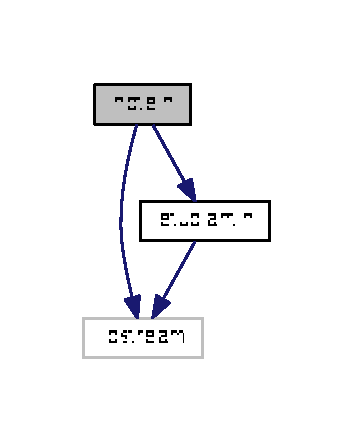
\includegraphics[width=169pt]{note_8h__incl}
\end{center}
\end{figure}
This graph shows which files directly or indirectly include this file\+:
\nopagebreak
\begin{figure}[H]
\begin{center}
\leavevmode
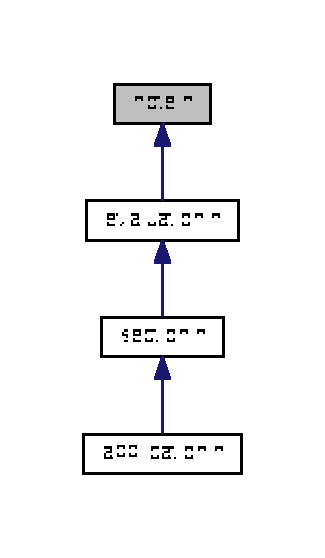
\includegraphics[width=156pt]{note_8h__dep__incl}
\end{center}
\end{figure}
\subsection*{Classes}
\begin{DoxyCompactItemize}
\item 
class \hyperlink{class_note}{Note}
\begin{DoxyCompactList}\small\item\em Permet de créer des notes en les lien avec les étudiants. \end{DoxyCompactList}\end{DoxyCompactItemize}


\subsection{Detailed Description}
\begin{DoxyAuthor}{Author}
Maxime I\+O\+R\+I 
\end{DoxyAuthor}
\begin{DoxyVersion}{Version}
0.\+1 
\end{DoxyVersion}

\hypertarget{section_8h}{\section{section.\+h File Reference}
\label{section_8h}\index{section.\+h@{section.\+h}}
}
{\ttfamily \#include $<$iostream$>$}\\*
{\ttfamily \#include \char`\"{}etudiant.\+h\char`\"{}}\\*
{\ttfamily \#include \char`\"{}evaluation.\+h\char`\"{}}\\*
Include dependency graph for section.\+h\+:
\nopagebreak
\begin{figure}[H]
\begin{center}
\leavevmode
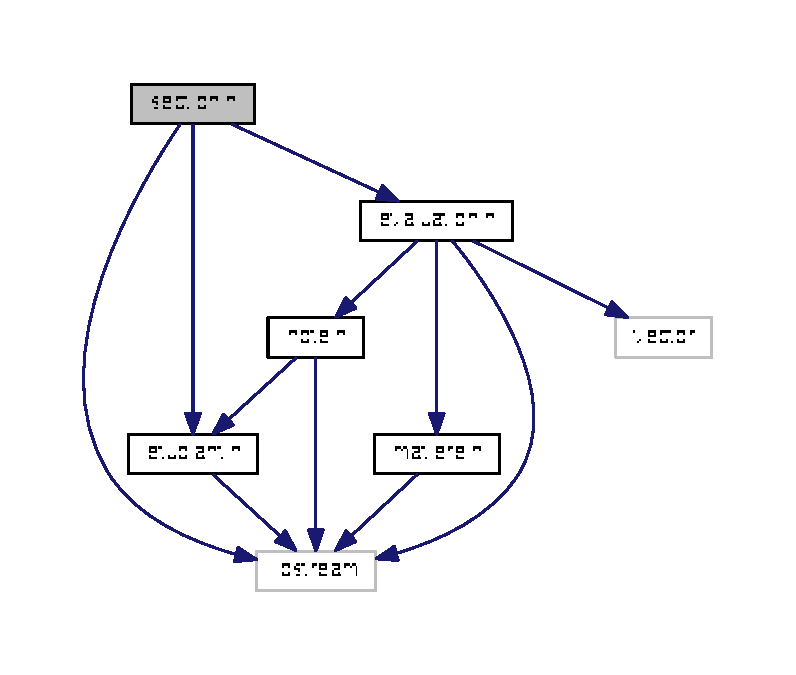
\includegraphics[width=350pt]{section_8h__incl}
\end{center}
\end{figure}
This graph shows which files directly or indirectly include this file\+:
\nopagebreak
\begin{figure}[H]
\begin{center}
\leavevmode
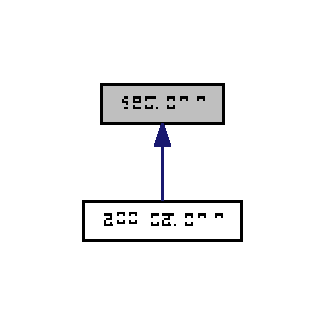
\includegraphics[width=156pt]{section_8h__dep__incl}
\end{center}
\end{figure}
\subsection*{Classes}
\begin{DoxyCompactItemize}
\item 
class \hyperlink{class_section}{Section}
\begin{DoxyCompactList}\small\item\em Permet le liens avec \hyperlink{class_section}{Section} pour en utiliser des éléments. \end{DoxyCompactList}\end{DoxyCompactItemize}


\subsection{Detailed Description}
\begin{DoxyAuthor}{Author}
Maxime I\+O\+R\+I 
\end{DoxyAuthor}
\begin{DoxyVersion}{Version}
0.\+1 
\end{DoxyVersion}

%--- End generated contents ---

% Index
\newpage
\phantomsection
\addcontentsline{toc}{chapter}{Index}
\printindex

\end{document}
